\begin{figure}[H] 
        \centering
        \begin{subfigure}[b]{0.45\linewidth}
            \centering
            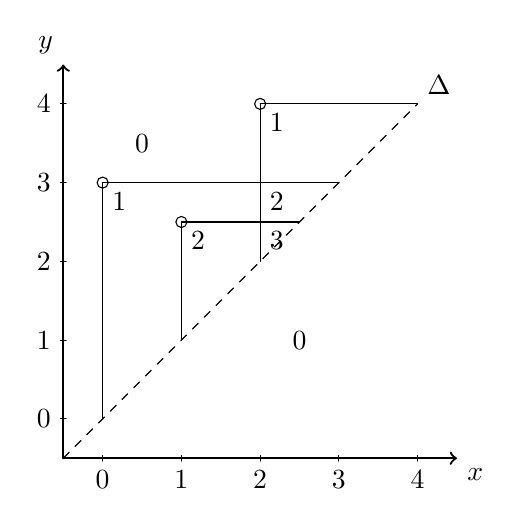
\begin{tikzpicture}[line cap=round, line join=round, x=1cm, y=1cm]
                
                \draw[thick,->] (0,0) -- (5,0) node[anchor=north west] {$x$};
                \draw[thick,->] (0,0) -- (0,5) node[anchor=south east] {$y$};
                \draw[dashed] (0,0) -- (4.5,4.5) node[above right] {$\Delta$};

                \draw (0.5 cm,1pt) -- (0.5 cm,-1pt) node[anchor=north] {0};
                \draw (1.5 cm,1pt) -- (1.5 cm,-1pt) node[anchor=north] {1};
                \draw (2.5 cm,1pt) -- (2.5 cm,-1pt) node[anchor=north] {2};
                \draw (3.5 cm,1pt) -- (3.5 cm,-1pt) node[anchor=north] {3};
                \draw (4.5 cm,1pt) -- (4.5 cm,-1pt) node[anchor=north] {4};

                \draw (1pt,0.5 cm) -- (-1pt,0.5 cm) node[anchor=east] {0};
                \draw (1pt,1.5 cm) -- (-1pt,1.5 cm) node[anchor=east] {1};
                \draw (1pt,2.5 cm) -- (-1pt,2.5 cm) node[anchor=east] {2};
                \draw (1pt,3.5 cm) -- (-1pt,3.5 cm) node[anchor=east] {3};
                \draw (1pt,4.5 cm) -- (-1pt,4.5 cm) node[anchor=east] {4};

                \draw (1.5, 3) circle (2pt) node[below right] {2};
                \draw (0.5, 3.5) circle (2pt) node[below right] {1};
                \draw (2.5, 4.5) circle (2pt) node[below right] {1};

                \draw (3, 1.5) node {0};
                \draw (1, 4) node {0};
                \draw (2.5, 3.5) node[below right] {2};
                \draw (2.5, 3) node[below right] {3};

                \draw (1.5, 3) -- (1.5, 1.5);
                \draw (1.5, 3) -- (3, 3);
                \draw (0.5, 3.5) -- (0.5, 0.5);
                \draw (0.5, 3.5) -- (3.5, 3.5);
                \draw (2.5, 4.5) -- (2.5, 2.5);
                \draw (2.5, 4.5) -- (4.5, 4.5);
                
            \end{tikzpicture}
            \caption{Rank function.}
        \end{subfigure}
        \hfill
        \begin{subfigure}[b]{0.45\linewidth}
            \centering
            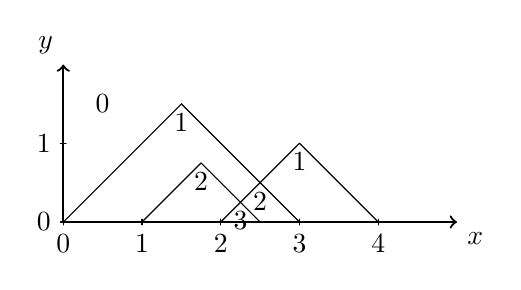
\begin{tikzpicture}[line cap=round, line join=round, x=1cm, y=1cm]
                
                \draw[thick,->] (0,0) -- (5,0) node[anchor=north west] {$x$};
                \draw[thick,->] (0,0) -- (0,2) node[anchor=south east] {$y$};

                \draw (0 cm,1pt) -- (0 cm,-1pt) node[anchor=north] {0};
                \draw (1 cm,1pt) -- (1 cm,-1pt) node[anchor=north] {1};
                \draw (2 cm,1pt) -- (2 cm,-1pt) node[anchor=north] {2};
                \draw (3 cm,1pt) -- (3 cm,-1pt) node[anchor=north] {3};
                \draw (4 cm,1pt) -- (4 cm,-1pt) node[anchor=north] {4};

                \draw (1pt,0 cm) -- (-1pt,0 cm) node[anchor=east] {0};
                \draw (1pt,1 cm) -- (-1pt,1 cm) node[anchor=east] {1};

                \draw (1.75, 0.75) node[below] {2};
                \draw (1.5, 1.5) node[below] {1};
                \draw (3, 1.0) node[below] {1};

                \draw (0.5, 1.5) node {0};
                \draw (2.5, 0.5) node[below] {2};
                \draw (2.25, 0.25) node[below] {3};

                \draw (1.75, 0.75) -- (1, 0);
                \draw (1.75, 0.75) -- (2.5, 0);
                \draw (1.5, 1.5) -- (0, 0);
                \draw (1.5, 1.5) -- (3, 0);
                \draw (3, 1.0) -- (2, 0);
                \draw (3, 1.0) -- (4, 0);
                
            \end{tikzpicture}
            \caption{Rescaled rank function.}
        \end{subfigure}
        \begin{subfigure}[b]{\linewidth}
            \centering
            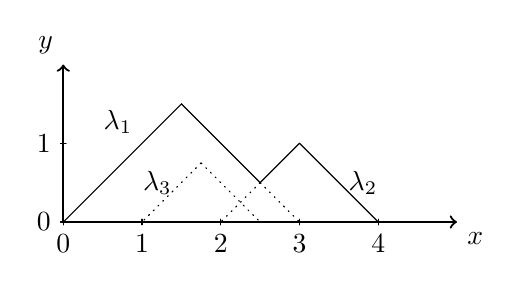
\begin{tikzpicture}[line cap=round, line join=round, x=1cm, y=1cm]
                
                \draw[thick,->] (0,0) -- (5,0) node[anchor=north west] {$x$};
                \draw[thick,->] (0,0) -- (0,2) node[anchor=south east] {$y$};

                \draw (0 cm,1pt) -- (0 cm,-1pt) node[anchor=north] {0};
                \draw (1 cm,1pt) -- (1 cm,-1pt) node[anchor=north] {1};
                \draw (2 cm,1pt) -- (2 cm,-1pt) node[anchor=north] {2};
                \draw (3 cm,1pt) -- (3 cm,-1pt) node[anchor=north] {3};
                \draw (4 cm,1pt) -- (4 cm,-1pt) node[anchor=north] {4};

                \draw (1pt,0 cm) -- (-1pt,0 cm) node[anchor=east] {0};
                \draw (1pt,1 cm) -- (-1pt,1 cm) node[anchor=east] {1};

                \draw[dotted] (1.75, 0.75) -- (1, 0);
                \draw[dotted] (1.75, 0.75) -- (2.5, 0);
                \draw (1.5, 1.5) -- (0, 0);
                \draw (1.5, 1.5) -- (2.5, 0.5);
                \draw[dotted] (2.5, 0.5) -- (3, 0);
                \draw (3, 1.0) -- (2.5, 0.5);
                \draw[dotted] (2.5, 0.5) -- (2, 0);
                \draw (3, 1.0) -- (4, 0);

                \draw (1, 1) node[above left] {$\lambda_1$};
                \draw (1.5, 0.5) node[left] {$\lambda_3$};
                \draw (3.5, 0.5) node[right] {$\lambda_2$};
                
            \end{tikzpicture}
            \caption{Persistence landscape.}
        \end{subfigure}
        \caption{Persistence landscape of a persistence diagram.}
        \label{fig:persistance-landscapes}
    \end{figure}